\section{Measuring the performance of the pipeline}\label{e2e}

The performance of the pipelined approach can be measured by assessing the alignments it produced. Because the number of theoretically possible alignments is massive there is no reference value to compare to. In fact, assessing the quality of an alignment is somewhat subjective because the size of the aligned chunks might be considered good by one person and bad by another person. We can however derive a few objective criteria that make up a good alignment:

\begin{enumerate}
	\item The aligned partial transcripts should cover the whole transcript
	\item The aligned partial transcripts should not overlap
	\item The aligned partial transcripts should be at the correct position (i.e. they should contain the text that is actually spoken)
\end{enumerate}

These criteria can be quantified with the following metrics (note the corellation\footnote{positive correlation: higher is better, negative correlation: lower is better}):

\begin{table}[!htbp]
	\centering
	\begin{tabular}{|l|l|l|l|}
		\hline
		\thead{criterion} & \thead{metric} & \thead{symbol} & \thead{correlation} \\
		\hline
		1 & \makecell[l]{length of text in ground truth that is not aligned vs. total length of the ground truth} & $C$ & negative \\ 
		\hline
		2 & \makecell[l]{length of overlaps in alignments vs. total length of alignments} & $O$ & negative \\ 
		\hline		
		3 & \makecell[l]{average Levensthein similarity between the transcript\\and the text in the ground truth corresponding to its alignment} & $D$ & positive \\ 
		\hline				
	\end{tabular}
	\caption{Metrics to evaluate the quality of alignments}
	\label{LM_evaluation}
\end{table}

These metrics can be weighted and reduced to a single number if necessary. Figure \ref{example_alignment} shows an example of an alignment. The sentence was split into speech segments by \ac{VAD} which were then aligned with the whole sentence (ground truth). Some speech segments were misaligned, resulting in an overlap. Some of the transcriptions contain mistakes. Note that the Levensthein Similarity ($ls(s_1, s_2)$) measures the similarity of two strings $s_1$ and $s_2$ as the normalized edit distance and is calculated as follows:

\begin{equation}
	ls(s_1, s_2) = 1 - \frac{ed(s_1, s_2)}{max \left(len(s_1), len(s_2), len(s_3)\right)}
\end{equation}

For $t_1=\text{i see}, t_2=\text{i c}, t_3 = \text{sad the blind men}, t_4 = \text{to his blind daughter}$ The metrics can be calculated as follows:

\begin{equation}
C = \frac{len(\text{i see})}{len(\text{i see i see said the blind man to his deaf daughter})} = \frac{5}{51} = 0.098
\end{equation}

\begin{equation}
\begin{split}
O & = \frac{len(\text{i see})}{len(\text{i see}) + len(\text{i c}) + len(\text{sad the blind men}) + len(\text{to his deaf daughter})} \\
 & = \frac{5}{5 + 3 + 17 + 20} = 0.11
\end{split}
\end{equation}

\begin{equation}
\begin{split}
D & = \frac{ls(\text{i see}, t_1) + ls(\text{i see}, t_2) + ls(\text{said the blind man}, t_3) + ls(\text{to his deaf daughter}, t_4)}{4} \\
 & = \frac{1 + 0.4 + 0.88 + 1}{4} = 0.82
\end{split}
\end{equation}

\begin{figure}
	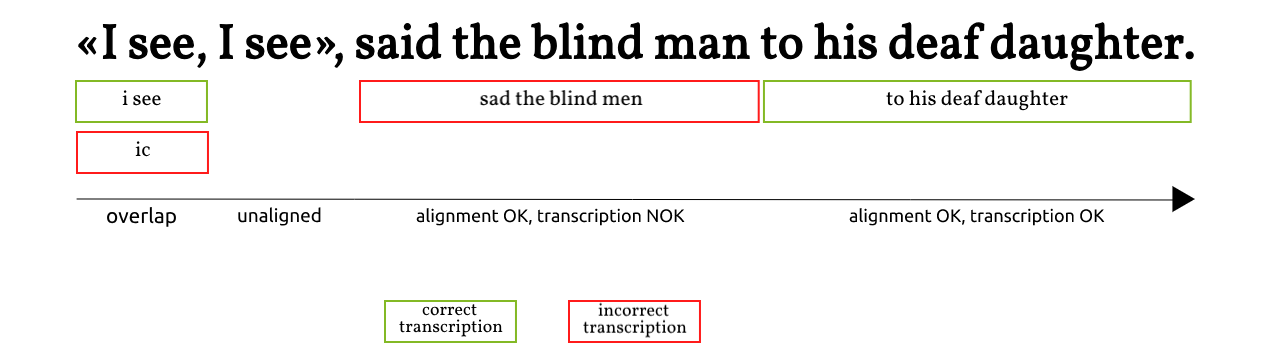
\includegraphics[width=\linewidth]{./img/example_alignment.png}
	\caption{Example for a partially correct alignment of parts of a sentence}
	\label{example_alignment}
\end{figure}